\section{Предложенный подход}
\label{sec:Chapter4} \index{Chapter4}

\subsection{Архитектура энкодера}

Было рассмотрено две разных архитектуры энкодера.

В качестве первого варианта будем использовать собственную архитектуру, состоящую из пяти сверточных слоев. Она обрабатывает 403.530 параметров. Обозначим данную архитектуру $N_1$. Она изображена подробно на рисунке ниже.

\begin{figure}[H]
    \center{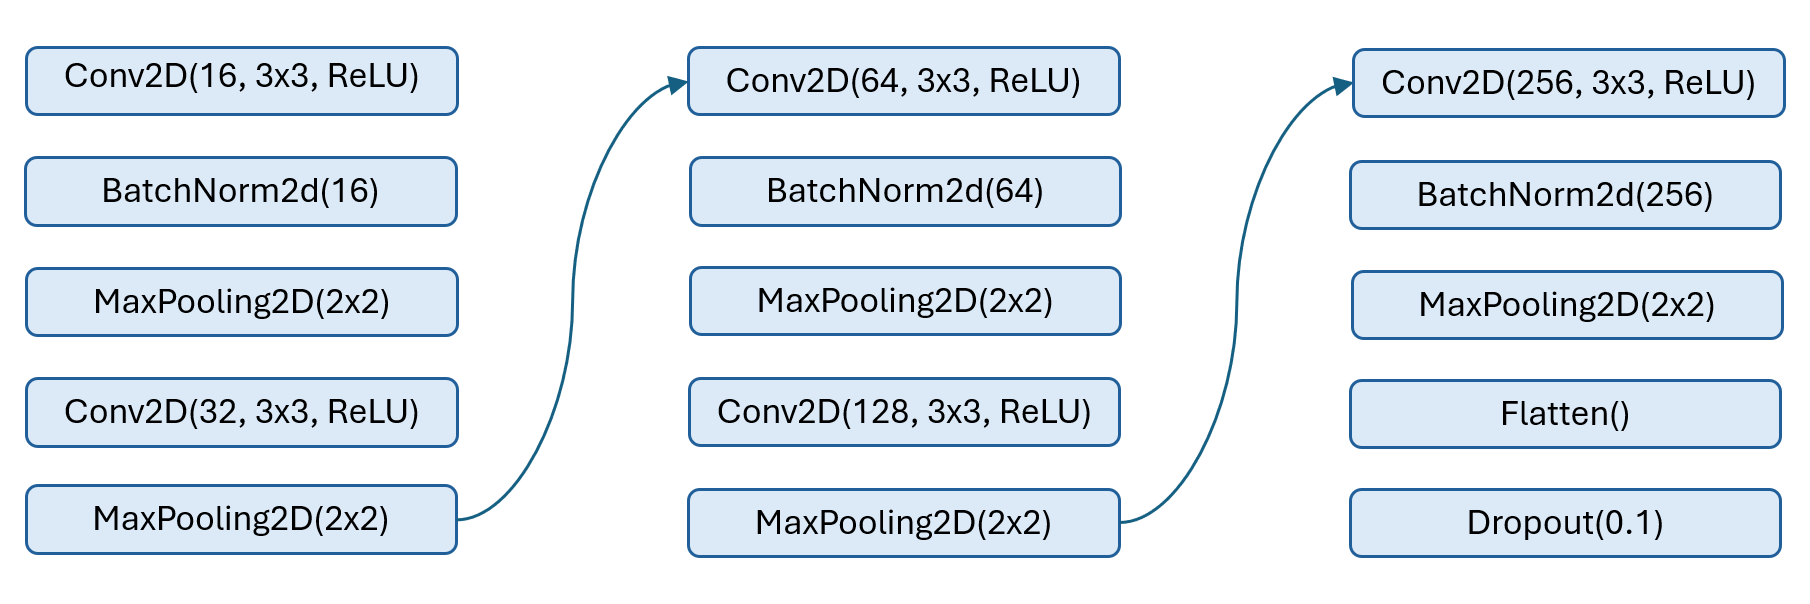
\includegraphics[height=5.5cm, keepaspectratio]{pictures/Encoder_1_arch.png}}
        \caption{Архитектура 1}
        \label{encoder_arch}
\end{figure} 

На выходе из нее получим эмбединги размером 256.

В качестве второго варианта была выбрана архитектура ResNet-18 \cite{ResNet18}. Она состоит из 17 сверточных слоев. Сначала идут первый сверточный слой с 64 фильтрами и слой MaxPooling. Далее идут 4 блока, каждый из которых состоит из 4 последовательных сверточных слоев и слоев Batch Normalization. В первом блоке каждый сверточный слой имеет 64 фильтра, в последующих блоках число фильтров увеличивается вдвое. Данная архитектура обрабатывает 11.681.896 параметров. Обозначим ее $N_2$. На выходе из нее получим эмбединги размером 512. 

Таким образом имеем две архитектуры энкодера, которые различаются глубиной и размером выходного пространства эмбедингов. 

\subsection{Проектор}

Для обучения модели также используется проектор, который последовательно соединяется с энкодером. Он представляет собой несколько полносвязных слоев. Для каждой архитектуры будем использовать три полносвязных слоя, каждый из которых имеет 1024 нейрона на выходе. Также после каждого слоя будем использовать Batch Normalization.
